%%%%%%%%%%%%%%%%%%%%%%%%%%%%%%%%%%%%%%%%%%%%%%
%                insertmeeting
% 1) Title (something creative & funny?)
% 2) Date (MM/DD/YYYY)
% 3) Location (ex. Hagerty High School)
% 4) People/Committees Present 
% 5) Picture 
% 6) Start Time & Stop Time (ex. 12:30AM to 4:30PM)
%%%%%%%%%%%%%%%%%%%%%%%%%%%%%%%%%%%%%%%%%%%%%%
\insertmeeting 
	{Fully Fed} 
	{03/24/22} 
	{Hagerty High School}
	{James, Jensen, Nathan, Ritam}
	{Images/RobotPics/robot.jpg}
	{2:30 - 4:30}
	
\hhscommittee{Software}
\noindent\hfil\rule{\textwidth}{.4pt}\hfil
\subsubsection*{Goals}
\begin{itemize}
    \item Implement a feedforward controller on our drivetrain motors. 

\end{itemize} 

\noindent\hfil\rule{\textwidth}{.4pt}\hfil

\subsubsection*{Accomplishments}
Currently, we control our motors using the Control Hub's built-in PID controller. The main advantage of this approach is speed. Running everything at a low-level in the REV Hub allows it to handle fine adjustments to the motors, helping them successfully execute the instructions that we give it. However, one thing we were considering was adding a dead wheel encoder to the robot. Having a dead wheel odometer would improve our localization accuracy during autonomous. Our choice to use only a single REV Hub limited our motor/encoder ports. We already need one encoder port for the turning wheel and one for the arm. Currently, the two motor encoders are used as part of the localization calculations. Replacing any of these encoders with the dead wheel odometer means that we would not be able to use the built-in velocity PID controller. One solution suggested in the "Learn Road Runner" website was to use feedforward tuning. Our mentor explained that feedforward tuning using a constant to determine the motor power needed to go a specific velocity. For example, we might know that we need to push a gas pedal down 3 inches to go 60 mph. To go a 20 mph, we should have to press the gas pedal down about 1 inch. Following the instructions, we were able to implement and tune a decent feedforward constant. After spending a little more time following the Road Runner sample tests, we decided that the feedforward controllers were acceptable. If and when we decide to mount the odometer wheel, we will fully switch to using feedforward control for the motors. 


\begin{figure}[htp]
\centering
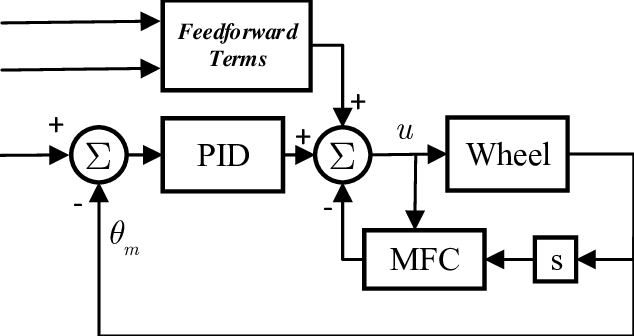
\includegraphics[width=0.95\textwidth, angle=0]{Meetings/March/03-24-22/03-24-22 1.png}
\caption{A graphic showing feedforward. While this image is a little complex, the idea of using a feedforward constant to adjust the motor power makes sense.}
\label{fig:032422_1}
\end{figure}

\begin{figure}[htp]
\centering
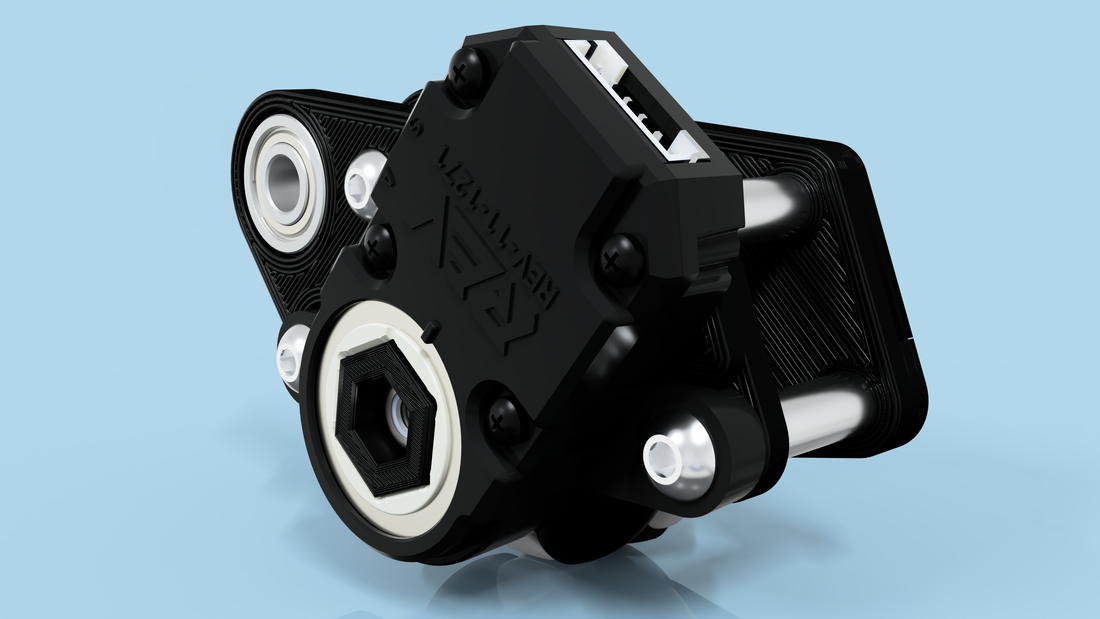
\includegraphics[width=0.95\textwidth, angle=0]{Meetings/March/03-24-22/03-24-22 2.png}
\caption{OpenOdometry was an open-source odometry system created for FTC teams. We plan to create a similar design for our own odometers.}
\label{fig:032422_2}
\end{figure}

\begin{figure}[htp]
\centering
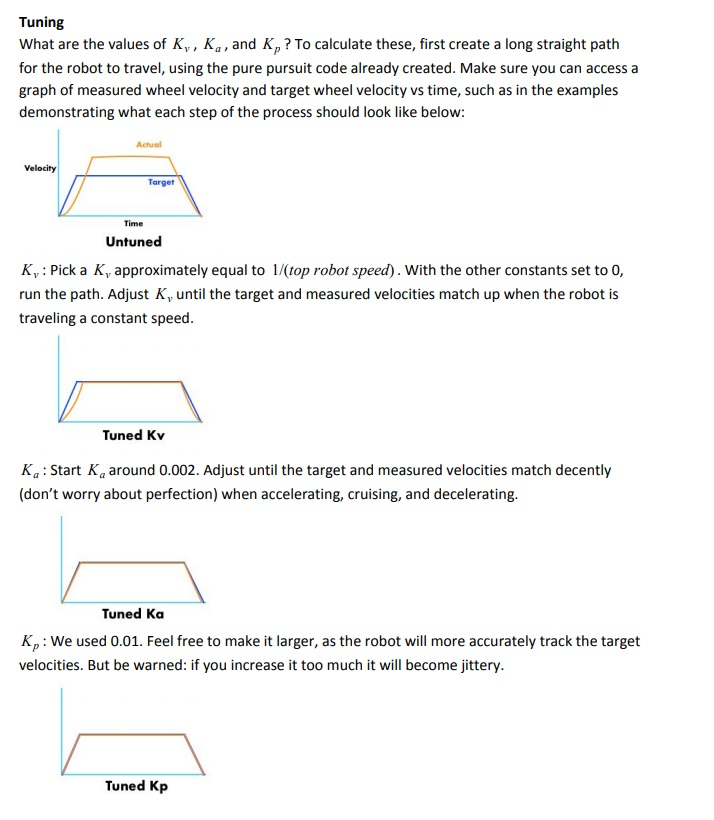
\includegraphics[width=0.95\textwidth, angle=0]{Meetings/March/03-24-22/03-24-22 3.jpg}
\caption{Guide from "Learn Road Runner" on tuning feedforward constants.}
\label{fig:032422_3}
\end{figure}



\whatsnext{
\begin{itemize}
    \item Design and mount an encoder wheel.
\end{itemize} 
}

